\documentclass[conference]{IEEEtran}
\IEEEoverridecommandlockouts
% The preceding line is only needed to identify funding in the first footnote. If that is unneeded, please comment it out.
\usepackage{cite}
\usepackage{amsmath,amssymb,amsfonts}
\usepackage{algorithm}
\usepackage{algorithmic}
\usepackage{graphicx}
\usepackage{textcomp}
\usepackage{xcolor}
\usepackage{booktabs}
\usepackage{multirow}  %表格跨行
\usepackage{threeparttable} %表格脚注
\usepackage{enumerate} %序数编号
\usepackage{indentfirst} %缩进
\usepackage{url} %引用网页
\usepackage{CJK}
\def\BibTeX{{\rm B\kern-.05em{\sc i\kern-.025em b}\kern-.08em
    T\kern-.1667em\lower.7ex\hbox{E}\kern-.125emX}}

\renewcommand{\algorithmicrequire}{ \textbf{Input:}} %Use Input in the format of Algorithm
\renewcommand{\algorithmicensure}{ \textbf{Output:}} %UseOutput in the format of Algorithm

\begin{document}
	\begin{CJK*}{UTF8}{song}
		
	%BibTex
	\bibliographystyle{plain}
	

\title{  从红楼梦看生存之道   \\
%\thanks{Identify applicable funding agency here. If none, delete this.}
}

\author{\IEEEauthorblockN{Kai Shan}
	
	 
\IEEEauthorblockA{\{shankai1995\}@hust.edu.cn/qq.com/gmail.com} 
}

\maketitle

\begin{abstract}
红楼梦中的夫人们是如何生存的??丫鬟们是怎样上位的??各自命运如何??
\end{abstract}

\begin{IEEEkeywords}
红楼梦, 夫人, 丫鬟
\end{IEEEkeywords}

\section{Background}
四大家族:贾史王薛

贾府的人物关系如Fig. \ref{jia_fu_structure}所示。
\begin{figure}[htbp]
	\centering
	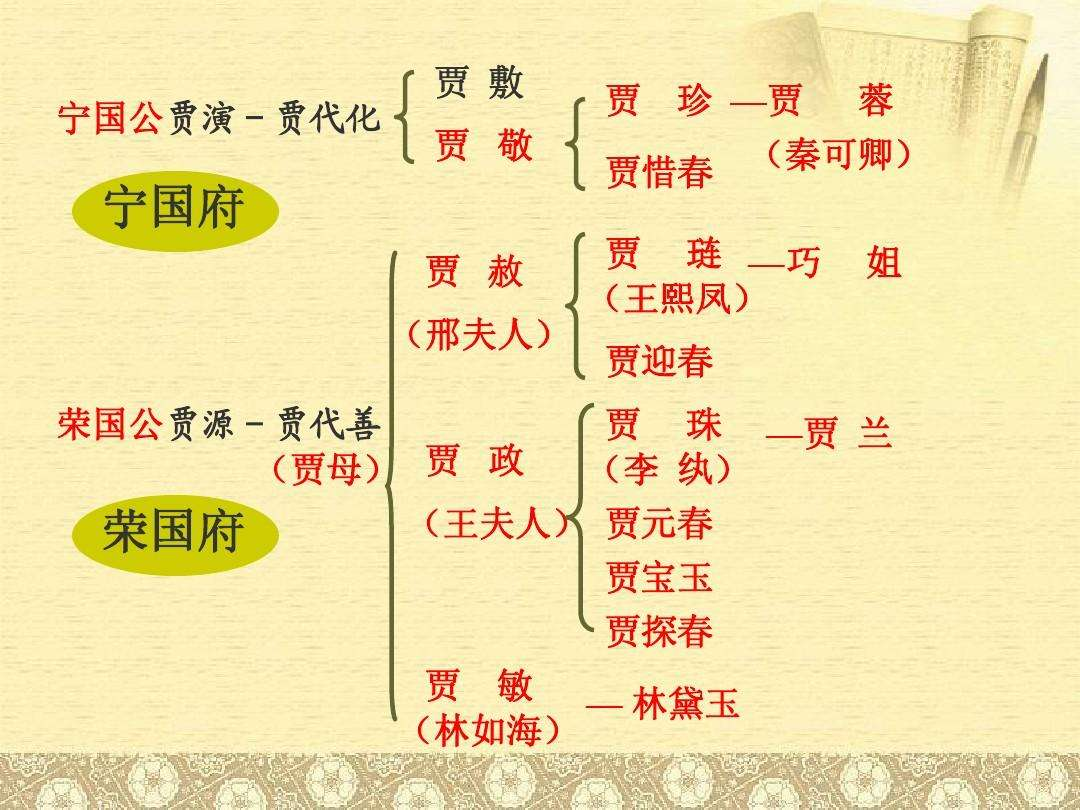
\includegraphics[scale=0.2]{jia_fu_structure.jpg}
	\caption{贾府任务关系图.}
	\label{jia_fu_structure}
\end{figure}



\section{夫人}
\subsection{王夫人}
\textbf{后台硬},没办法。贾府绝对的大总管。金陵王氏子弟。荣国府一把手贾政的老婆。

王夫人,\textbf{面慈心狠}。大家闺秀,彬彬有礼,不能乱了礼法,掉了身份。有事赵姨娘上,由她打滚撒泼,王夫人当老好人。等到所有人都收拾的差不多了,狡兔死,走狗烹;飞鸟尽,良弓藏;敌国破,谋臣亡,收拾赵姨娘。	

多给丫鬟们小恩小惠。

\subsection{王熙凤}
王熙凤,王夫人侄女,王熙凤。后台硬+能干(流产还管家呢),贾府第一劳模。

\textbf{有管理能力} 典型例子,办秦可卿的丧事。(1)扬刀立威,开会迟到的仆人,二十大板,相应的管家口一个月工钱。谁主管谁负责

\subsection{周姨娘和赵姨娘}
都是贾政的小老婆。

周姨娘\textbf{不生事},王夫人也不动她。\textbf{(*,这个可以考虑)}

赵姨娘,王夫人的陪嫁丫鬟。打滚撒泼她上,王夫人的枪。狡兔死,走狗烹;飞鸟尽,良弓藏;敌国破,谋臣亡,下场可想而知。\textbf{单纯的当一只舔狗是不行的。}

\subsection{邢夫人}
贾赦的继室,娘家后台不硬。无一儿半女。

啥都没有,只能依靠老公。疯狂为老公介绍小老婆。

疯狂找机会咸鱼翻身。邢夫人看王夫人姑侄那是相当之不顺眼。邢夫人是大老爷贾赦的夫人,贾政是二老爷,邢夫人是大儿媳,可是诸事由王夫人说了算。另外,王熙凤是邢夫人的儿媳,可,王熙凤就没把这婆婆当回事。丫鬟傻大姐,捡到了一只绣春囊,上绘春宫图,有伤教化。邢夫人想借此收拾王熙凤()王熙凤老公贾琏好色,很可能是他的东西)。王夫人借此彻查,不仅还了王熙凤清白,并且借此良机,clear了所有的异己()代表人物,晴雯)。

虽然失败了。但是人生能有几回搏?\textbf{(人生能有几回搏??*)}

\subsection{尤夫人}
贾珍的继室,娘家后台不硬。

贾珍跟儿媳妇秦可卿有一腿(扒灰),贾府上下人尽皆知,秦可卿死的时候,贾珍哭的可伤心了。尤氏自知地位不稳,忍耐。并且尤氏带来尤氏双姐妹,尤二姐尤三姐跟贾珍贾蓉父子不清不楚。最终尤三姐自杀。

\textbf{尤氏为稳固地位牺牲了自己妹妹,感觉这人什么都可以牺牲了}

\subsection{李纨}
贾宝玉早夭的哥哥贾珠的媳妇。儿子贾兰。

不争风吃醋,李纨文学水平很高,一心扑在诗社上。一心放在业余爱好上。

\textbf{一心想当文艺女青年,可惜贾兰死后,也死去了}

\subsection{小结}
顺成人,逆成仙,都在其中颠倒颠。无论豪门寒门,都会面临着同样的问题的。





\section{丫鬟}

\subsection{晴雯}
看不上王夫人的小恩小惠。王夫人很生气,后王夫人借抄检大观园之机弄死了。

王夫人愿望晴雯,晴雯激烈反抗,绝食。王夫人讲绝食多天的晴雯赶回娘家()理由和充分,说晴雯有传染病,为大家伙着想),晴雯当天气病而死。中间有一段很凄美的\textbf{宝玉探晴雯},宝玉偷偷摸摸背着王夫人去探望晴雯,\textbf{晴雯把自己贴身的肚兜给了宝玉},“冷雨凄风不可听,乍分离处最伤情;钏松怎奈重添病,腰瘦何堪再减容”。

\textbf{晴雯任性、傲气} 敢跟贾宝玉顶嘴。

\subsubsection{晴雯撕扇}

\textbf{起因} “偏生晴雯上来换衣服,不防又把扇子失了手跌在地下,将股子跌折。”试想宝玉此时心内糟糕之极,一腔无名无有宣泄之所,这晴雯恰于此时将扇跌折。若在平时,以宝玉宽仁之心必不计较,此时晴雯就成了倒霉的出气筒了。宝玉因叹道:“蠢才,蠢才!将来怎么样?明日你自己当家立事,难道也是这么顾前不顾后的?”
这里宝玉借机发作一番,而且对象是自己房中的一个丫鬟,而且就跌扇一事而言,言之亦未太过,不算故意挑晴雯的不是。此时若换做袭人,麝月等其余丫头或许就顺着宝玉的口气,认个错或者顾左右而言它,就遮掩过去了。偏偏晴雯是块暴炭,立马反唇相讥。这下宝玉房内炸锅了,连带来劝架的袭人也落了个灰头土脸。最后,宝玉一定要回了太太去,至袭人一干丫鬟跪下求情才罢。

\textbf{经过} 这一场吵闹之后,宝玉房中诸人都很不自在。适时黛玉过来调侃了几句,缓和了一下房中的紧张气氛,其他人或许就揭过去了。然而,当事人宝玉和晴雯内心的芥蒂仍存着呢。然后是呆霸王请吃酒,归来时已带了几分酒意了。注意,从拌嘴至醉归,宝玉和晴雯都还没说过和解的话,两人内心还别扭着呢。然后还是宝玉主动寻求和解,:“你的性子越发惯娇了。早起就是跌了扇子,我不过说了那两句,你就说上那些话。说我也罢了,袭人好意来劝,你又括上她,你自己想想,该不该?”。能和宝玉处一个屋内,也算晴雯之福了。然后宝玉说出了一番对物用的态度,“你爱打就打,这些东西原不过是借人所用,你爱这样,我爱那样,各自性情不同。比如那扇子原是扇的,你要撕着玩也可以使得,只是不可生气时拿他出气。就如杯盘,原是盛东西的,你喜听那一声响,就故意的碎了也可以使得,只是别在生气时拿他出气。这就是爱物了。”这里宝玉一再主动寻求和解,直到说出一番物用的道理:高兴就好!晴雯何等冰雪聪明,马上打蛇上杆,“既这么说,你就拿了扇子来我撕。我最喜欢撕的。”甚至宝玉夺过麝月的扇子,递与晴雯,在宝玉的嘻笑和纵容下,晴雯毫无顾忌,也撕了几半子。

\textbf{结果} 宝玉和晴雯因吵架心中所存的芥蒂荡然无存了。竟此一吵一撕一笑之后,两人的关系应该更好了吧!

其一、毫无疑问刻画了晴雯天真幼稚,张扬率性的性格特征,也为其后来的遭遇埋下伏笔。其二、反映了宝玉对物用的态度,只要自己开心就要,不要生气时拿着器物来出气,至于是否物尽其用,人尽其才到在其次了。其三的确有遥应褒姒笑狼烟之典,侧写晴雯之貌美,设若把晴雯换做袭人或麝月一干人等,恐怕宝玉无此一番言论。

\textbf{出身低贱的人是没有人性的资本的!!!找准自己位置}
\textbf{要学会示弱,以弱胜强,以柔克刚}

\subsection{鸳鸯}
\textbf{对领导忠心耿耿}

鸳鸯死心塌地跟着贾母,鸳鸯也是贾母唯一信任的人。

贾赦硬让邢夫人去向贾母讨鸳鸯做他的小老婆,还亲自对鸳鸯的哥哥说:“自古嫦娥爱少年,他必定嫌我老了,大约是恋着少爷们,多半是看上宝玉,只怕也有贾琏。果有此心,叫她早早歇了心,我要她不来,此后谁还敢收?此是一件。第二件,想着老太太疼她,将来自然往外聘做正头夫妻去。叫她细想,凭她嫁到谁家去,也难出我的手心。除非她死了,或是终身不嫁男人,我就服了她。”  \textbf{贾赦收鸳鸯未必不是看上了鸳鸯是老太太心腹这一点。}

鸳鸯死活不同意,在贾母死后自杀。

\subsection{袭人}
王夫人担心自己的宝贝疙瘩贾宝玉被其他丫鬟迷的五迷三道,无心学习,派袭人监视。贾宝玉初试云雨情,就是和袭人。王夫人默许,可是袭人会把宝玉的一切报告给王夫人。宝玉发现之后,逐袭人出贾府,嫁给优伶蒋玉菡。

“枉自温柔和顺,空云似桂如兰;堪羡优伶有福,谁知公子无缘”

\textbf{错在间谍身份暴露了,找个老实人嫁了,结局也算是可以了}

\textbf{鸳鸯和袭人这种,省却了决策负担,命运也掌握不在自己手里。}

\subsection{小红}
\textbf{想上位,咸鱼翻身}

\textbf{有切实可行的目标}。填贾宝玉的房没戏,找到了贾宝玉的侄子,贾云。贾云虽然穷点,但是正经贵族,人长得也帅。

小红和贾芸一见钟情,便丢下红罗帕私定终身(创造机会接近贾芸,\textbf{天上不会掉馅儿饼,要主动出击}),在贾府没落之时和贾芸结为伉俪,相比较而言,她的结局是比较美好的,不像司棋也有意中人,却落了个碰墙而死。

\subsection{平儿}
王熙凤的陪嫁丫头,后给琏二爷填房,地位不改变,仍是丫鬟待遇,贾琏两口子的出气筒,平儿逆来顺受,\textbf{老老实实,本本分分},还救了主母王熙凤的女儿巧姐(王熙凤死后,贾府没落之时,有人想将巧姐嫁给外藩王爷,赚钱,平儿将巧姐交给刘姥姥带出大观园,贾琏知道后,觉得平儿可以,扶正,成为大夫人)。

\section{Conclusion}
1. 独立自主。夫人丫鬟都是依附于男人的,存在人身依附关系,很难活出自我的。

2. 有能力。 一定要求自己的独到之处。

3. 但行好事,莫问前程。

4,本本分分,安分守己。

5. 中心耿耿,但是不能把鸡蛋放在一个篮子里。否则,风险很大。

6. 什么都没有,什么都不是的舔狗,最后一无所有。

7. 和光同尘。以弱胜强,以柔克刚。



\bibliographystyle{IEEEtran}
%Refremces 最后的参考文献
%\bibliography{sk_bib}
\end{CJK*}

\end{document}
